\documentclass[11pt,a4paper]{article}
\usepackage[latin5]{inputenc}
\usepackage[english]{babel}
\usepackage{amsmath}
\usepackage{amsfonts}
\usepackage{amssymb}
\usepackage{graphicx,subfig}
\usepackage{placeins}
\usepackage{gensymb}


\begin{document}

\section{Eroding and dilating}
We have made the text on the Africa map bolder by eroding with a 3 by 3 rectangle as a structuring element, as seen on Fig. \ref{fig:a2a}. We have then cleared out the text by dilating the image three times with the same rectangle structuring element as before, as seen on Fig. \ref{fig:a2a}. For the map outline, we cancelled out the text as before, then we eroded three times to revert the effects of dilation on the map outline, then we copied the image, eroded again and subtracted the copy from the image. The result can be seen in Fig. \ref{fig:a2a}.
\begin{figure}%
\centering
\subfloat[][The original image]{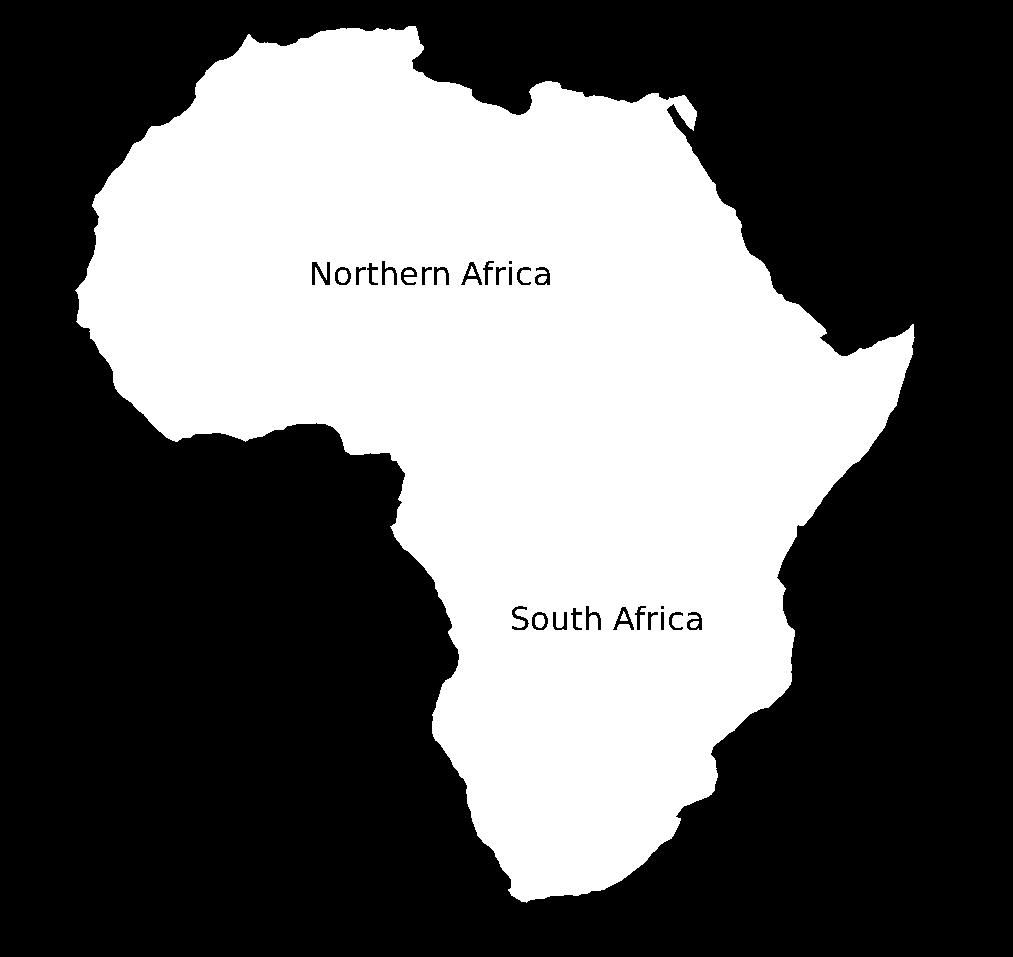
\includegraphics[scale=.3]{data/africa.png}}
\quad
\subfloat[][Eroded]{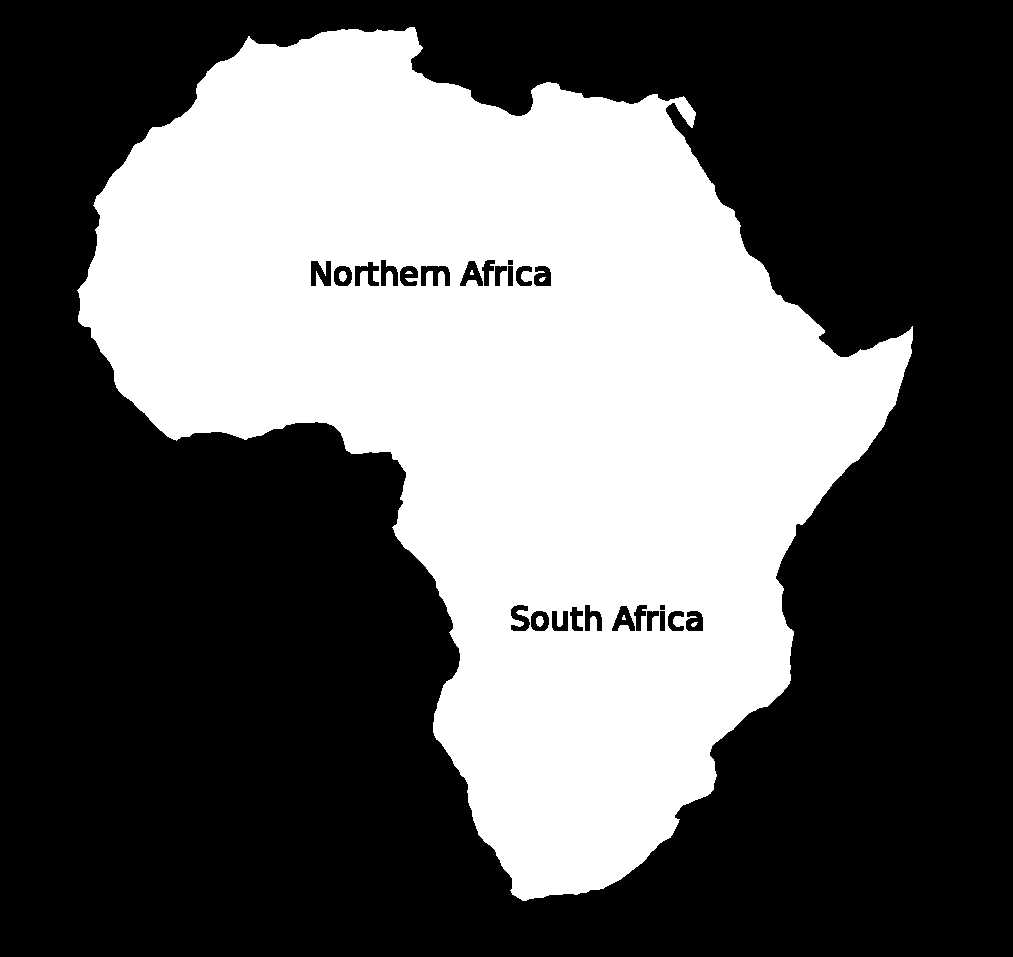
\includegraphics[scale=.3]{data/res/eroded.png}}
\quad
\subfloat[][Dilated]{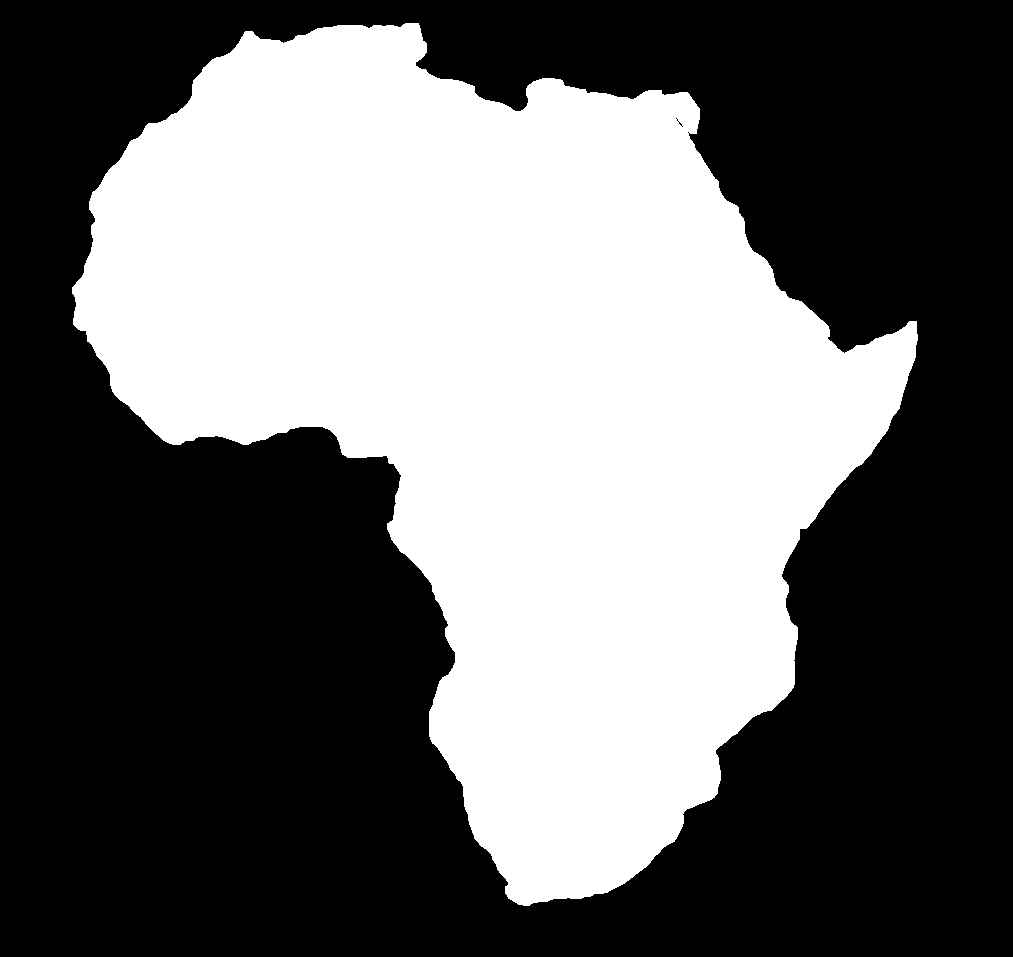
\includegraphics[scale=.3]{data/res/dilated.png}}
\quad
\subfloat[][Outlines through erosion and subtraction]{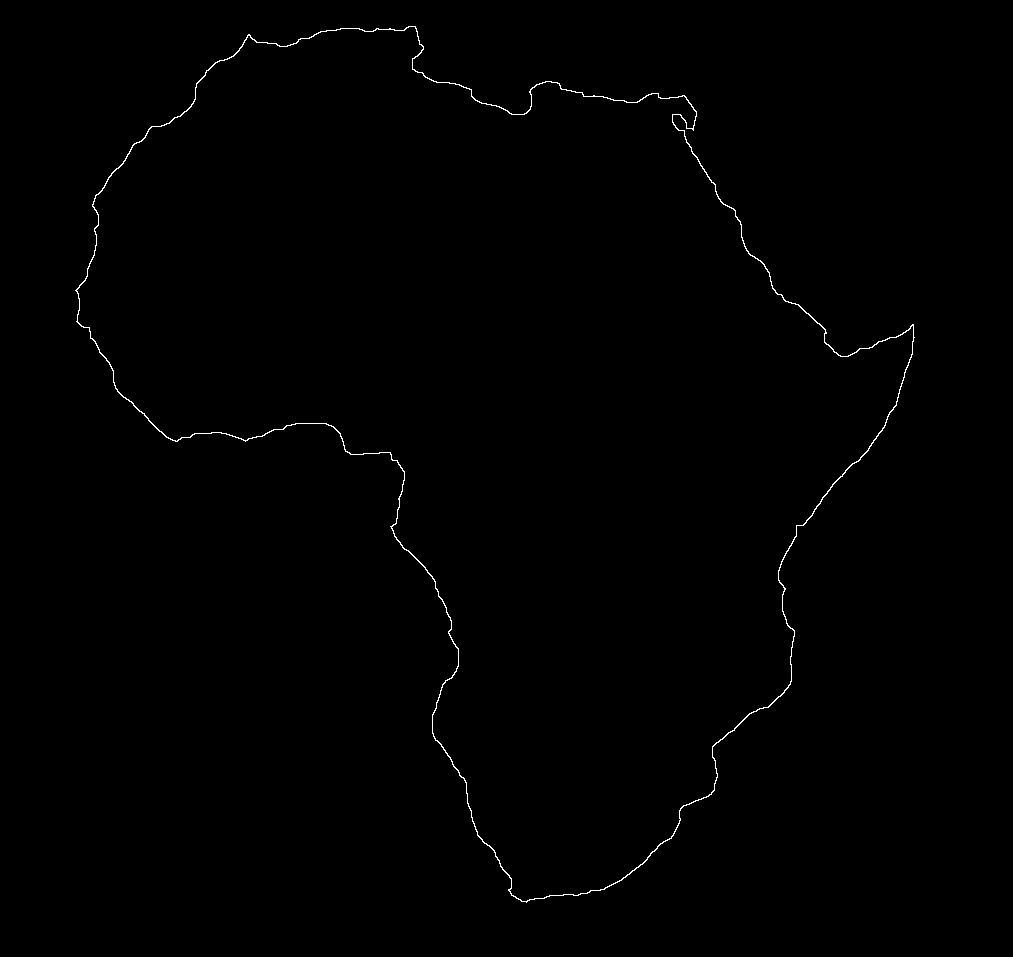
\includegraphics[scale=.3]{data/res/border.png}}
\quad
\caption{Erosion and dilation on a binary image}%
\label{fig:a2a}%
\end{figure}

\section{Opening and closing}
By using opening with a 9 by 9 circle as a structuring element, we were able to separate the dots from the lines in Fig. \ref{fig:a2b}. For the cells image, we have found that applying the same opening operation with a 7 by 7 circle after thresholding is very well suited for finding blobs above a certain size, in this case the larger cell bodies. We have also applied closing to the circles image with the same disk shaped structuring element and have discovered that this operation makes the line circles around the filled circles disappear.
Making the structuring element bigger (17 by 17) will slowly get rid of the smaller dots and in the end as it gets large enough (33 by 33) it will cancel all the dots in the image.

\begin{figure}%
\centering
\subfloat[][The original dotsandlines image]{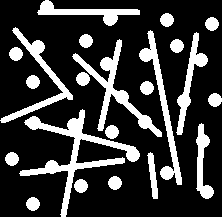
\includegraphics[scale=.3]{data/dotsandlines.png}}
\quad
\subfloat[][Separated]{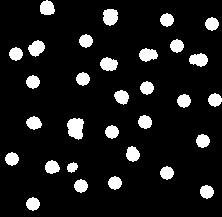
\includegraphics[scale=.3]{data/res/dots.png}}
\quad
\subfloat[][Original Cells]{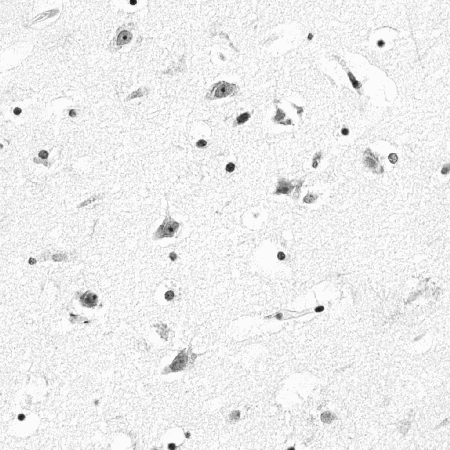
\includegraphics[scale=.3]{data/cells.png}}
\quad
\subfloat[][Thresholded Cells]{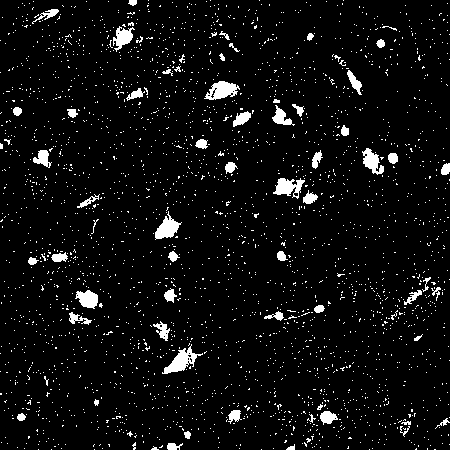
\includegraphics[scale=.3]{data/res/cells_thresh.png}}
\quad
\subfloat[][Cell body detected by opening]{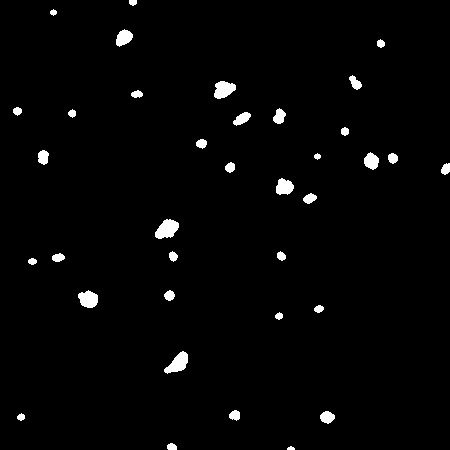
\includegraphics[scale=.3]{data/res/dots1.png}}
\quad
\subfloat[][Circles original]{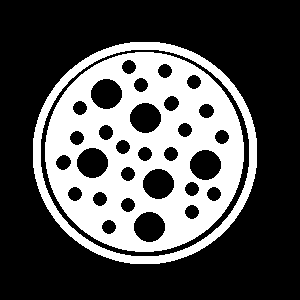
\includegraphics[scale=.3]{data/circles.png}}
\quad
\subfloat[][Circles closed]{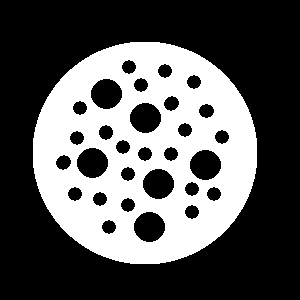
\includegraphics[scale=.3]{data/res/circles_closed9.png}}
\quad
\subfloat[][Circles closed larger element]{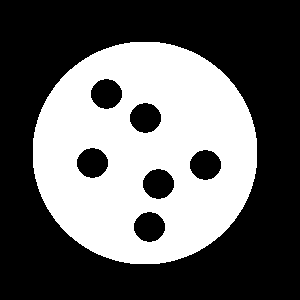
\includegraphics[scale=.3]{data/res/circles_closed17.png}}
\quad
\subfloat[][Circles closed even larger element]{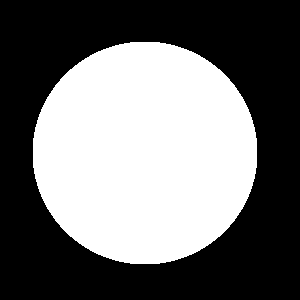
\includegraphics[scale=.3]{data/res/circles_closed33.png}}
\quad
\caption{Opening and closing}%
\label{fig:a2b}%
\end{figure}

\section{Advanced}
We have taken the house image (Fig. \ref{fig:a2c}) and tried to implement an edge detection by using the morphological gradient with a 3 by 3 cross as structuring element. After thresholding at 60, the lines are clearly visible on the output image. Compared to Canny it performs worse, since Canny also tries to suppress non-maxima and attempts to connect different parts of a line.
For corner detection, we have added the absolute value of the morphological gradient with a horizontal line as structuring element to the same with a vertical structuring element. After thresholding, regions where both gradients are strong will stay and thus we have found a corner.

\begin{figure}%
\centering
\subfloat[][The original image]{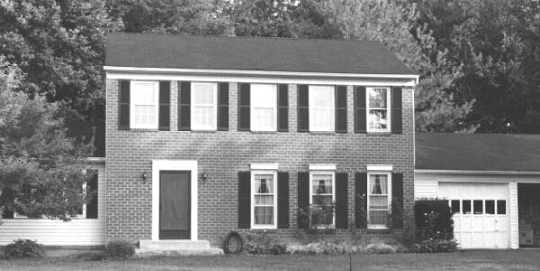
\includegraphics[scale=.3]{data/house.png}}
\quad
\subfloat[][Thresholded morphological gradient]{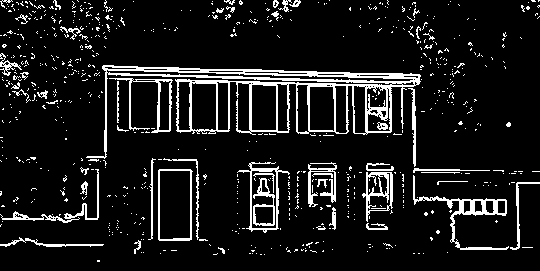
\includegraphics[scale=.3]{data/res/grad.png}}
\quad
\subfloat[][Canny]{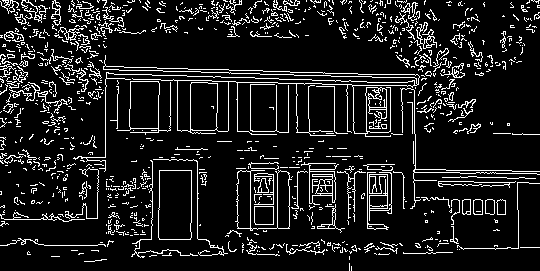
\includegraphics[scale=.3]{data/res/canny.png}}
\quad
\subfloat[][Corner detection]{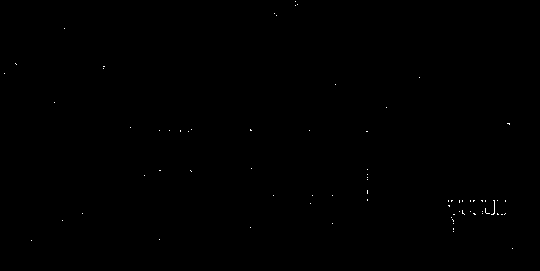
\includegraphics[scale=.3]{data/res/corners.png}}
\quad
\caption{Advanced morphological operations}%
\label{fig:a2c}%
\end{figure}

\end{document}

